\documentclass[10pt,a4paper]{article}
\usepackage[UTF8]{ctex}
\usepackage{amsmath}
\usepackage{amsfonts}
\usepackage{amssymb}
\usepackage{float}
%\usepackage{clrscode}
\usepackage[]{algorithm2e}
\usepackage{graphicx}
% Set the margin of document.
\usepackage[top=10mm, bottom=12.5mm, left=12.5mm, right=12.5mm]{geometry}
\usepackage{longtable}
\usepackage{float}
\renewcommand\figurename{图}
\renewcommand\tablename{表}
\title{实验数据的平滑滤波(Smoothing)}
\author{袁略真\\3130103964\\生物信息学\\浙江大学}
\begin{document}
\maketitle

\section{平滑滤波的意义}
通常,物理规律$y=f(x)$在某一区间内应该是连续光滑的. 然而实际测量中,受到随机噪声的影响导致数据$(x_i,y_i)$叠加上噪声信号.这种噪声通常是随机的.为了将规律展示出来,在某些应用场合下可以使用平滑(smoothing)的方法将噪音信号滤去.然而在科学研究中应当慎用这种方法,因为平滑可能造成信号的失真.

之所以能使用平滑的方法滤去噪声,是因为噪声通常有一定的概率统计性质.平滑是使用一定的模型在一些数据点上以最小均方差逼近原始数据.不同平滑方法的区别在于模型的选择以及数据点的选取.

设有如下观测数据:
\begin{table}[H]
\caption{观测数据}
\centering
\begin{tabular}{|c|c|c|c|c|c|c|}
\hline 
x & $X_0$ & $X_1$ & ... & $X_i$ & ... & $X_N$ \\ 
\hline 
y & $Y_0$ & $Y_1$ & ... & $Y_i$ & ... & $Y_N$ \\ 
\hline 
\end{tabular} 
\end{table}
当考虑处理$(X_i,Y_i)$数据点时,考虑以该点为中心的5个数据点,并将自变量用t表示:
\begin{table}[H]
\caption{五数据点}
\centering
\begin{tabular}{|c|c|c|c|c|c|}
\hline 
t & -2 & -1 & 0 & 1 & 2 \\ 
\hline 
y & $Y_{i-2}$ & $Y_{i-1}$ & $Y_i$ & $Y_{i+1}$ & $Y_{i+2}$ \\ 
\hline 
\end{tabular} 
\end{table}

处理方法以如下两种为例.
\subsection{五点线性平滑}
这种方法使用线性模型:
$$y_{i+t}=A_0+A_1t$$
以如下最小均方差:
$$min(\sum\limits_{t=-2}^{2} [(A_0+A_1t)-y_{i+t}]^2)$$
算得$A_0,A_1$,用$A_0$代替$Y_i$即可.

\subsection{五点三次平滑}
这种方法使用三次方程:
$$y_{i+t}=A_0+A_1t+A_2t^2+A_3t^3$$
以如下最小均方差:
$$min(\sum\limits_{t=-2}^{2} [(A_0+A_1t+A_2t^2+A_3t^3)-y_{i+t}]^2)$$
算得$A_0,A_1,A_2,A_3$,用$A_0$代替$Y_i$即可.

\section{计算结果}
分别以N=$1~50$,获得N个随机数取平均.运行n=1000次,对这1000个数据计算平均值的标准偏差.

获得50组平均值的标准偏差,对该数据集使用平滑处理,得到的结果用图形展示如下:

\begin{figure}[H]
\centering
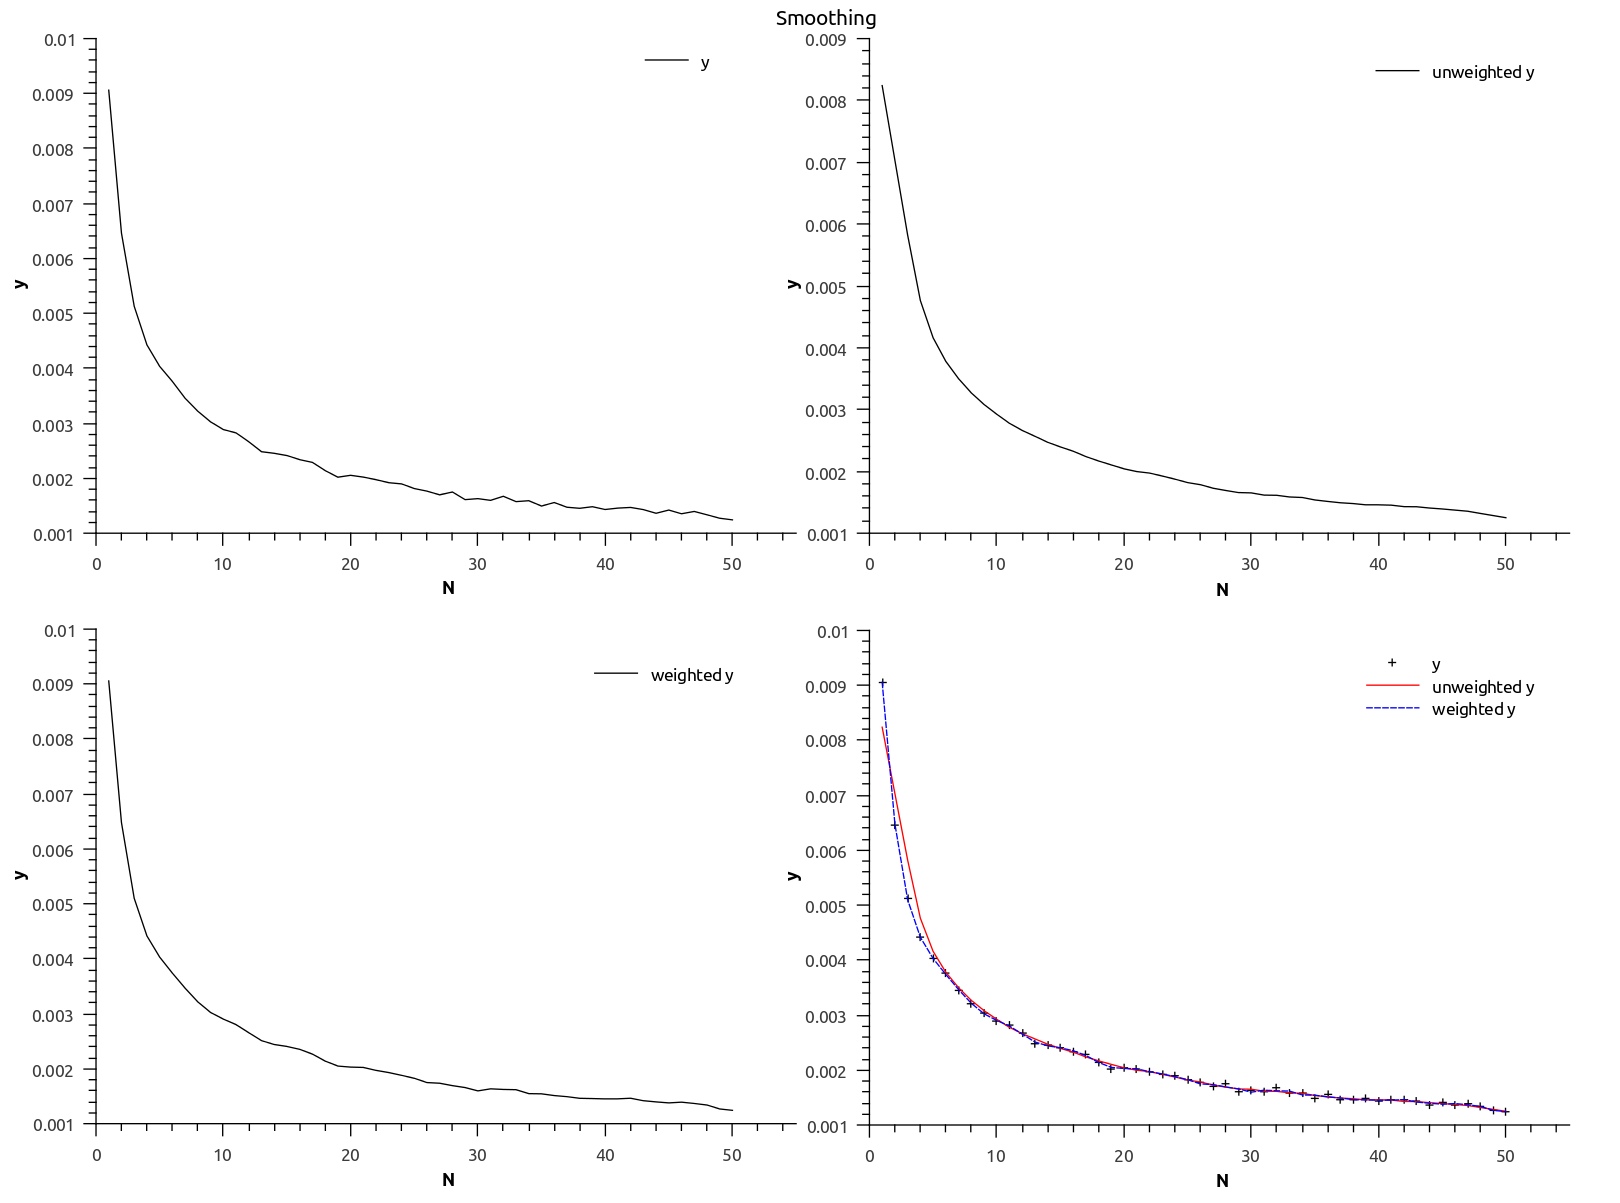
\includegraphics[width=\textwidth]{../result/Graph2.png}
\caption{平滑处理之前(左上),平滑处理后(右上,左下),以及3个数据集在一幅图中的情况.右上的平滑使用五点线性平滑.左下的图使用五点三次平滑.}
\end{figure}

就光滑效果,五点线性平滑更好.
\end{document}